\testCom
{%Номер задачи
	3.204
}
{%Условие
	условие
}
{%Дано
	дано
}
{%Найти
	найти
}
{%Решение
	%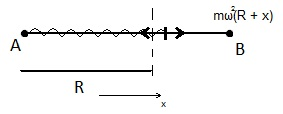
\includegraphics[height=30mm]{3_33.jpg}\\
	Если в струне установились полуволны, значит $\nu = 50$Гц - собственная частота струны.\\
	Из соотношения $\upsilon = \sqrt{\frac{F}{\rho_l}} \Rightarrow F = \upsilon^2 \rho_l$\\
	Очевидно, что $\rho_l = \rho S = \rho \frac{\pi d^2}{4}, \rho$ - объёмная плотность\\
	$\upsilon = \lambda \nu$ из условия $l = \eta \frac{\lambda}{2} \Rightarrow \lambda = \frac{2 l}{\eta}$\\
	таким образом $F = \rho \pi d^2 \cdot \frac{l^2}{\eta^2} \nu^2$\\
}

